{\color{teal!90}\chapter{XMG6780A-V2 Firmware Update}\label{cap:XMG6780A-V2}}

\AddToShipoutPictureBG*{%
  \AtPageUpperLeft{%
    \raisebox{-\height}{%
      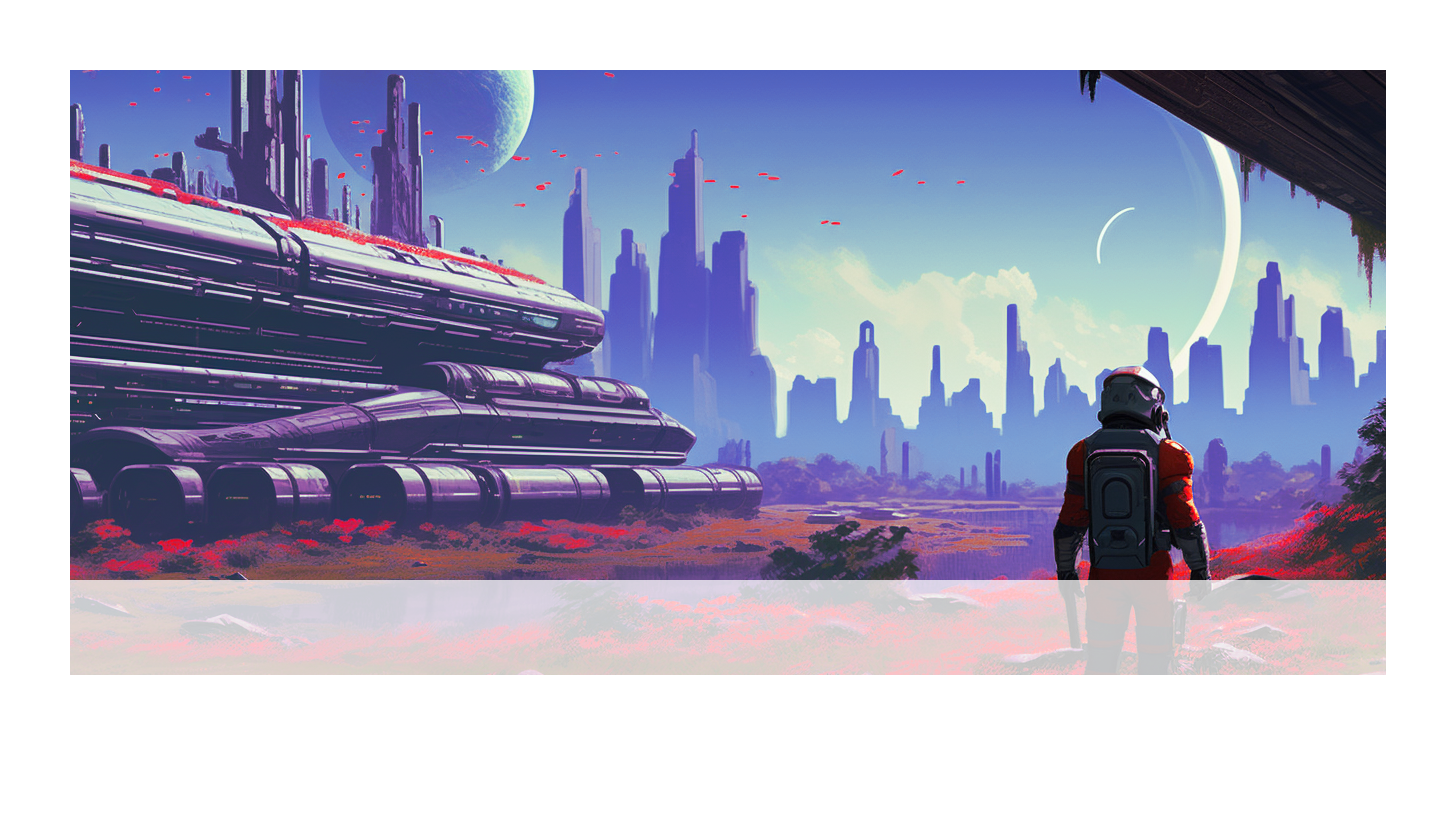
\includegraphics[width=\paperwidth]{./chapters/XMG6780A-V2.png}%
    }%
  }
}

\minitoc% Creating an actual minitoc mini lista contenuti


\section{XMG6780A-V2 Firmware}

After installing the \href{https://www.dropbox.com/scl/fi/razk4d533kkrign0e0kd1/wetransfer_new-firmware_2023-09-04_0553.zip?rlkey=jrls1bpkyo93ul3i0t1nokexu&dl=0}{XMG6780A-V2} firmware on the device, new customization options arise, including the ability to replace the default Launcher3 with a custom launcher. The limitations outlined in Cap. \ref{cap:resetting} encountered in the firmware originally present on the device at the time of Akhter's purchase on 08-08-2023, can be overcome by using the XMG6780A-V2 firmware.

\medskip
Once the custom launcher is configured as the default home, the issue of infinite boot-loop upon reboot is resolved. However, a problem might arise where the default launcher continues to appear despite the HOME action redirecting to the actual new custom launcher.

To resolve this issue, it's necessary to disable the default launcher3 using \cmd{\color{BrickRed}pm disable} for the \texttt{\color{BrickRed}com.xbh.launcher.overlay} and \texttt{\color{BrickRed}com.xbh.launcher} apps.

However, using the \texttt{\color{BrickRed}pm disable} in Android app would require root access. So we can either install the root firmware the Havistouch team provided us with, or we can use the \texttt{\color{BrickRed}hide} counterpart of \textbf{\color{BrickRed}devicepolicymanager} within our \emph{Taishan Tweaker} custom launcher.

With the intention of developing a new functional launcher, the idea is to create an in-app setup sequence. This sequence will guide us through the various steps that must be executed in the correct order:

\subsection{In-App Setup Sequence}

\begin{enumerate}
    \item set IP to \ipnum{\taishanIP}
    \item install \gls{shizuku} from the USB Kioxia drive
    \item install \gls{termux} from \href{https://github.com/danieledellacioppa/termux-app}{my fork}
    \item \cmd{adb connect \taishanIP}
    \item \faPlayCircle Install Taishan Tweaker
    \item Execute \cmd{adb shell dpm set-device-owner}\footnote{\label{dpm-enable-command} The full syntax is \texttt{\color{BrickRed}adb -s 192.168.11.207 shell dpm set-device-owner com.akhter.taishantweaker/.receivers.admin.AdminReceiver}}
        \begin{enumerate}
            \item{Now launch manually\footnote{\label{manually}Sometimes, the app remains on without the need for manual launch. This change occurred because, since 2023-10-05, the AdminReceiver triggers the SetupActivity to launch the MainActivity, whereas previously it used to directly launch the MainActivity leading the SetupActivity to crash systematically.} the Taishan Tweaker app}
            \item{Allow access to foto and media}
            \item{\faIcon{map-marker-alt} Location needs to be allowed at all times, otherwise it's a security risk. So for the time being, part of the setup involves going in Developer Settings and allowing this permission and set it to {\color{Bluetto}\faIcon{toggle-on} \android{Allow all the time}}}
            \item{The background will turn white.\footnote{\label{background-white} I've noticed that sometimes it doesn't and goes straight to the default one}}
        \end{enumerate}
    \item Set the custom launcher as default
        \begin{enumerate}
            \item The \faImage background will be the default one. Meaning the wall0.jpg which has index 0 in the list of wallpapers held by MyWallpaperManager
        \end{enumerate}
    \item Apply Tweaks
        \begin{enumerate}
            \item Always check that the Default Launcher option doesn't show Launcher3 anymore
            \item Also check Office WPS is actually gone
        \end{enumerate}
    \item Reboot
    \item Stop the Kiosk or enable everything via SAF
    \item Create a Google account
    \begin{enumerate}
        \item{This means going to Settings -> System -> About -> Click 10 times on About label -> Debug -> Enable Google Play Services}
        \item Open Google Play Store \faGooglePlay
        \item Might crash the first time
        \item Open again and log in with
        \begin{enumerate}
            \item{email: npcguillemruiz@gmail.com}
            \item{password: j4m3sbondwillr3turn}
        \end{enumerate}
        \item You should see the list of apps that are available for download
        \item {\color{BrickRed}\faWrench} Update all the apps via the Play Store
    \end{enumerate}
    \item Go back to the Taishan Tweaker and Install the keyboard\faKeyboard
    \begin{enumerate}
        \item{This will open the Play Store \faGooglePlay \ on the Gboard page}
        \item{\faPlayCircle Install}
        \item Don't open it yet
    \end{enumerate}
    \item Set Gboard as the default keyboard\faKeyboard
    \item Disable SmartIME
    \item Reboot
    \item Go back to the Taishan Tweaker and you should be all set to ship it to the customer
\end{enumerate}

\section{Replicating the CTOUCH Launcher Solution}

Since this touchscreen is different, rebuilding everything is necessary. The Android 8 CTOUCH Solution cannot be reused as it proves to be too unpredictable. The steps for this replication could be as follows:

\begin{enumerate}
    \item Setting up the Kiosk mode.
        \begin{enumerate}
            \item Maintaining an updated list of allowed packages.
                \begin{enumerate}
                    \item{Looking at violations attempt in Lock Task can give me the name of the package I want to enable}
                    \item{Translating the whole admin module is too much. I'm just doing an app\_lister button for now}
                \end{enumerate}
            \item onResume the kioskmode is set everytime. Is this what I want? \footnote{\label{onResume} for example when I launch the calculator the onResume is called and the kioskmode is set again.}
            \item Refer to the \textbf{central entity}\footnote{\label{central-entity} The central entity is a Class encapsulating a DevicePolicyManager, named MyDevicePolicyManager, which is injected via Dagger2.} that stores the complete list (as discussed in Section~\ref{sec:kiosk}) to prevent unexpected behavior.
            \item Ensure that the \textbf{central entity}\footref{central-entity} is the only one used throughout the program, as opposed to using a naked devicePolicyManager, which could lead to inconsistency. But because Dagger2 works only with activities we can't inject directly in AdminReceiver. It needs to pass through the MainActivity
        \end{enumerate}
    \item Configuring \gls{saf}\footnote{\label{SAF} Secure Access Framework} to enable challenge password functionality.
          \begin{enumerate}
              \item USBDetector now detects ProductID and VendorID
              \item UsbAttachReceiver that listens for Broadcasts when a USB is attached or detached. This class tries to put loginComplete to false when a USB is detached. This is not working yet. It'll be useful for \gls{saf}
              \item \gls{saf} is making use of shared preferences in a weird way...maybe I need a \textbf{central class} to handle all the shared preferences
          \end{enumerate}
    \item Creating a recyclerView to display applications.
    \item Disabling the sidebar\footnote{\label{sidebar} Ensuring that apps are only accessible via TaishanTweaker}
        \begin{enumerate}
            \item {\gls{navisettings} is the name of the floating sidebar that can be disabled. The question is: can I create a floating bar from my app to create/handle events like onBackPressed, Recents, PowerOFF, Reboot, etc..?}
            \begin{enumerate}
                \item{\gls{navisettings} might be actually part of the system and I could adjust the look accordingly. This way I can post-pone recyclerView implementation. Also I won't have to create a floating bar to navigate.}
            \end{enumerate}
        \end{enumerate}
    \item Adding buttons in the \gls{ui} to control Wi-Fi\faWifi, Bluetooth\faBluetooth \footnote{\label{blue-not-needed} Invoking the getInstalledApplications(PackageManager.GET\_META\_DATA) method on an instance of the PackageManager class, returns a list of all the installed applications. This list includes the Bluetooth app. This means that Bluetooth can be disabled already without having to write any code.}, screenshots, and USB\faHdd \ functionality.
    \begin{enumerate}
        \item We should consider registering a BroadcastReceiver to \emph{android.net.conn.CONNECTIVITY\_CHANGE} to detect when the device is connected to the internet. At the moment, this is being done by launching a service that shuts the wifi periodically. This is not ideal.
        \begin{enumerate}
            \item{We found a package called \textbf{com.android.networkstack} that is both responsible for the Wi-Fi and the Ethernet. We can disable it. There will be a reboot. And both Wi-Fi and Ethernet will be disabled.}
        \end{enumerate}
        \item Bluetooth is not needed. It can be disabled already by disabling \emph{com.android.bluetooth} in the \textbf{Package Disabler}.
        \item Screenshots is part of the USB button. I need to split it.
        \item USB has a proper button now to enable/disable it. I need to add the functionality to take screenshots.
    \end{enumerate}
    \item Make the app lighter by removing unnecessary code. There are several performance issues that need to be addressed.
\end{enumerate}

\clearpage
\subsection{Kiosk}
\label{sec:kiosk}

To ensure proper functionality, it's essential to have a \textbf{central entity}\footref{central-entity} that globally stores the complete updated list of allowed packages. Otherwise, running the command at line \ref{lockArray} of the Listing \ref{lst:kioskfun} in the future may result in packet loss and lead to unexpected behaviors that are challenging to debug.

\lstinputlisting[language=Kotlin,linewidth=0.8\linewidth,caption={Kiosk Function}, label=lst:kioskfun, escapechar=\%]{./chapters/code/kioskfun.kt}

\subsection{Hiding packages}

Using the devicePolicyManager to hide packages can create problems. Here comes the list of packages that you shouldn't hide:

\begin{itemize}
    \item android
    \begin{enumerate}
        \item This package if allowed you'll be able to shutdown during Kiosk mode. If you disable it, you won't be able to shutdown at all. I'll keep it away from the list of packages to hide.
    \end{enumerate}
    \item android.ext.services
        \begin{enumerate}
            \item The system remains stable if you disable it. The issue is, this is a module that updates framework components for core Android OS functionality. These components include services for managing notifications, text auto-complete matching strategies, storage cache, and other services that run continuously. The module is updatable, meaning it can receive updates to functionality outside of the normal Android release cycle. Is autocompletion a requirement for the user? If so, then we can't disable it. For now I'll keep it away from the list of packages to hide.
        \end{enumerate}
    \item android.ext.shared
        \begin{enumerate}
            \item The system remains stable if you disable it. I don't what it does but it's probably related to the previous package. I'll keep it away from the list of packages to hide.
        \end{enumerate}
    \item com.android.apps.tag
        \begin{enumerate}
            \item The system remains stable if you disable it. It's the NFC app? I'll keep it away from the list of packages to hide.
        \end{enumerate}
    \item com.android.backupconfirm
        \begin{enumerate}
            \item The system remains stable if you disable it. It's belonging to the dialog popping up when initiating adb backup, and which does nothing but asking you to confirm whether the remotely triggered backup should be executed (and if you want to protect it with a password). I'll keep it away from the list of packages to hide.
        \end{enumerate}
    \item com.android.bips
        \begin{enumerate}
            \item The system remains stable if you disable it. It's the Bluetooth Input Profile Service. I'll keep it away from the list of packages to hide.
        \end{enumerate}
    \item com.android.bluetoothmidiservice
        \begin{enumerate}
            \item The system remains stable if you disable it. It's the Bluetooth MIDI Service. I'll keep it away from the list of packages to hide.
        \end{enumerate}
    \item com.android.bluetooth
        \begin{enumerate}
            \item This packet seems like it's doing the same thing I've done on CTOUCH Android 8. It's a service that runs in the background and it's responsible for the Bluetooth functionality. If you disable it, you won't be able to turn on Bluetooth again. I'll definitely keep it as an option for the user to enable/disable.
        \end{enumerate}
    \item com.android.cameraextensions
        \begin{enumerate}
            \item The system remains stable if you disable it. In low light scenarios, the camera app will automatically switch to night mode. I'll keep it away from the list of packages to hide.
        \end{enumerate}
    \item com.android.systemui
        \begin{enumerate}
            \item The system goes black.
            \item You can't unhide it since it'll give you the outpout shown at line n. \ref{systemui_out} of the Listing \ref{lst:unhidesystemui}.
            \item It remains hidden anyway. One way to recover is via \cmd{\color{BrickRed} adb shell reboot recovery}
        \end{enumerate}
\end{itemize}

\lstinputlisting[language=bash,linewidth=0.8\linewidth,caption={Unhiding SystemUI}, label=lst:unhidesystemui, escapechar=\%]{./chapters/code/unhide_android_systemui}

\begin{itemize}

    \item com.android.settings
    \item com.android.providers.set
    \item com.android.providers.settings
    \item com.android.providers.userdictionary
    \item com.android.providers.contacts
    \item com.android.providers.media
    \item com.android.providers.downloads
    \item com.xbh.share
        \begin{enumerate}
            \item This is AirgoCast and takes advantage when the app crashes so for security reasons it's disabled for now
        \end{enumerate}
\end{itemize}







